\section{Project Definition}\insertloftspace
\setcounter{figure}{0}\setcounter{table}{0}

\subsection{Market study}

At the request of Mr. Kedziora, we began by conducting a \gls{ms}\footnote{Analyze, understand and measure the real functioning of the forces at work in a market.} market study. Even if he had already done it, it allowed us to better understand the expectations of our customers, and the possible difficulties. It was also a way to have the point of future users of our product.

\bigbreak
Mr. Kedziora wanted to sell the robot in the United States. We focused on this region even if we also studied the situation in France. For that we contacted farmers by asking them questions about : 
\begin{itemize}[noitemsep]
    \item The size of their farms
    \item The method of collection and the duration
    \item The points of attention to picking apples
    \item The type of soil
    \item The difficulties encountered in finding personnel
    \item The interest for the use of robots: motivation and fear.
    \item The possible price.
\end{itemize}

It turned out that only the big farms ($\bg$ 50 acres) were interested. Indeed, out of the twenty or so farms that we contacted, more than 80\% were having difficulty recruiting, this phenomenon increased with the Covid crisis. This is not the case for small farms because they work mainly with local people and need fewer people. Thus, all the large farms were in favor of using robots. However, they warned us about the current existence of autonomous robots and the need to distinguish themselves. According to them, the big disadvantages of robotization today are the price of access and maintenance. A remote-controlled robot can answer their request by reducing the cost. However, our robot must keep the advantages of autonomous robots: the possibility to be used 24h and reducing the number of employees needed. The continuous work is a primordial point because the robots are generally slower than the humans but can have a better output on a complete day. Finally, technical characteristics were also put forward: Not too much pressure on the fruit, the ability to drive on potentially muddy dirt roads, and dimensions to respect.

\bigbreak
We also went directly on the spot to visit orchards in order to have a better vision of all these constraints and to be able to better discuss with the farmers. It was thus of great help to write the specifications. 

\subsection{State of the art}

At the same time as we were doing the market research, we were also interested in what was currently being done. There are several robot solutions for picking up fruit. All of them, however, use artificial intelligence and are autonomous. Partly because of this, their price is generally very high. Many of these are also relatively young and have not yet gained the full confidence of users. A good example is the FFRobotics robot that was in late development in February 2019 but the cost of a machine is between \$300,000 and \$350,000. They finally launched their robot in July 2022, 6 months after our project. Similarly, the company Abundant Robotics also created a robot capable of picking up apples by sucking them. However, this one had to close in July 2021 because of a lack of customers.
\begin{figure}[ht]
    \centering
    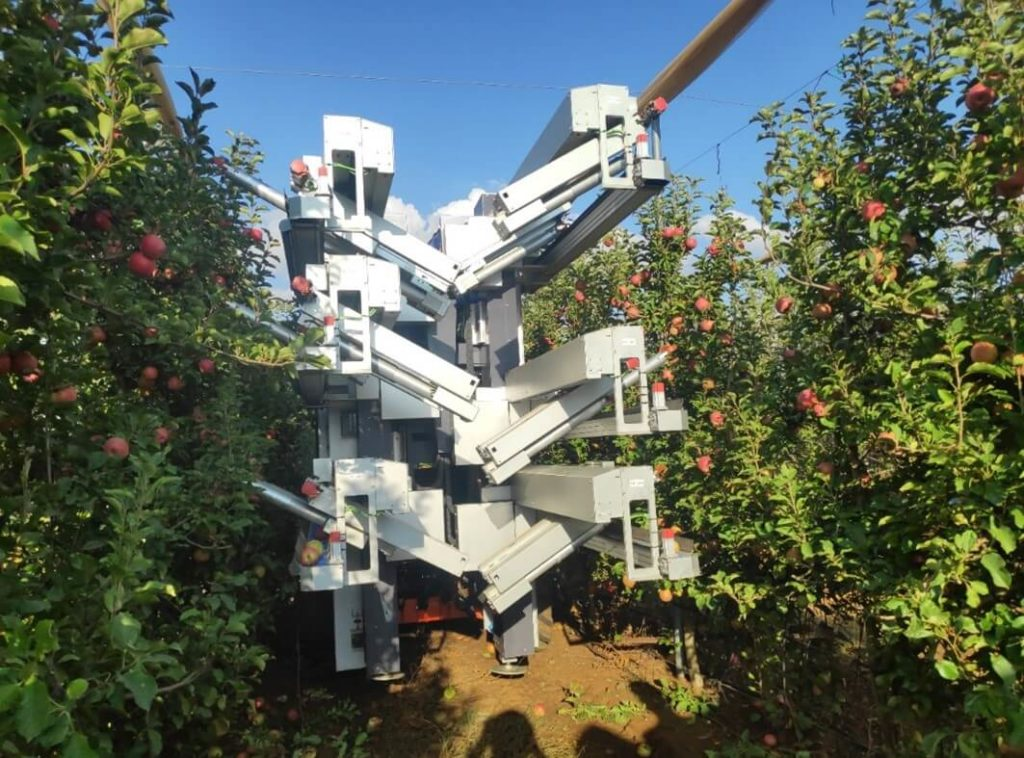
\includegraphics[width=0.8\textwidth]{Images/Section01/ffRobotics.png}
    \caption{FFRobotics robot}
    \label{fig:ffRobotics}
\end{figure}

\bigbreak
As the farmers we spoke with told us, the price is the main reason why they do not invest in these solutions. Our objective is to propose a solution using relatively easy and inexpensive manufacturing techniques. The desire of our customer to use a remote operator is also a way to reduce the design time and therefore the cost of the project. These robots are also usually very bulky and we want to try to reduce their size to move them more easily.

\bigbreak
Finally, there are also studies that we could rely on. For example, the article by Joseph Davidson \cite{Davidson-2016-126540} gives the ways to pick apples with a robot and indicates the maximum pressure that can be exerted.

\subsection{Definition}

After conducting a market study and a state of the art, we were able to redefine the project. Initially, our client wanted us to design and manufacture a complete robot: a base and an arm. His main constraint was the flexibility of the robot to be able to adapt to other tasks and thus be used throughout the year. As we have seen when we did the state-of-the-art, many bases already exist and are relatively cheap. Moreover, Mr. Kedziora also wanted us to start from a blank page in order not to be influenced by what already exist. It would have taken too much time to focus on everything. With his agreement, we decided to focus on the arm, the hand, and the control system. 

\bigbreak
Indeed, the main point of this project was to recover the fruits without damaging them. The hand was therefore the central element to distinguish us. We also kept the creation of the arm because the robot had to have a low cost and we wanted to imagine the least expensive design. For the same reason, we also kept the implementation of the control system. 

\bigbreak
Finally, during the project and facing the difficulties we encountered, we also evolved the project during the year. The apple harvest became the cherry tomato harvest. This allowed us to reduce the dimensions of our robot while keeping almost all the constraints we had to respect. We were therefore able to make all the prototypes with the "traditional" tools of the school. We were also able to meet the flexibility criteria required by our client. 

\subsection{Scope statement}

Following this, we made a \gls{ss}\footnote{Defines the purpose of the project, the stages of its realization, and the elements necessary to carry it out}. These studies as well as the evolution of the project allowed us to estimate the expectations and constraints. 

\bigbreak
\noindent The general cases of use that we could list are the following : 
\begin{itemize}[noitemsep]
    \item Picking up
    \item Storage of fruits
    \item Storage of robots
    \item Cleaning of the robot
    \item Recycling (not treated in the following)
\end{itemize}

We then made an "\gls{octopus}\footnote{Represents the relationship between a product and its environment}" which illustrates the links between the different functions: 
\begin{figure}[ht]
    \centering
    \includegraphics[width=0.8\textwidth]{Images/Section01/octopus\_diagram.png}
    \caption{Octopus diagram}
    \label{fig:octopus}
\end{figure}

\bigbreak
Only the main functions are presented here, the entire specification can be retained in appendix \ref{section:CDC}. The main function is to be as efficient as a human over a day. Thus the arm will have to retrieve a tomato in less than 10s. 

\begin{table}[ht]
    \centering  
    \begin{tabular}{|p{3cm} | p{3cm} | p{3cm} | p{3cm} |} 
        \hline
        \textbf{Principal Function} & \textbf{Appreciation criteria} & \textbf{Level} & \textbf{flexibility} \\ [0.5ex] 
        \hline\
        PF 1: Be at least as efficient as a human & harvest duration & less than 10s & F2 \\ 
        \hline
        PF 2: Picking tomatoes & The tomatoes are detached & 80\% of standard orchards are collect & F1 \\
        \hline
        PF 3: Controlling the robot & Pick tomatoes & get 80\% of tomatoes & F2 \\
        \hline
        PF 4 Control the robot remotely  & User can be in other place & 500m distance & F2 \\
        \hline
    \end{tabular}
    \caption{Principal functions extract}
\end{table}
\FloatBarrier

\bigbreak
The main constraint function is to reach all the tomatoes. To measure this, we want our robot to be able to reach 80\% of the tomatoes in a standard orchard. 

\begin{table}[H]
    \centering    
    \begin{tabular}{|p{3cm} | p{3cm} | p{3cm} | p{3cm} |} 
        \hline
        \textbf{Constraint Function} & \textbf{Appreciation criteria} & \textbf{Level} & \textbf{flexibility} \\ [0.5ex] 
        \hline\
        CF 1: Keeping tomatoes intact & Forces exerted & less than 5N & F1 \\ 
        \hline
        CF 2: Avoid branches and tomatoes & Precision & relative gap\less1cm & F1 \\
        \hline
        CF 3: Be easy to pilot & User feeling & Learn time\less2h & F2 \\
        \hline
    \end{tabular}
    \caption{Constraint functions extract}
\end{table}
